\documentclass[tikz,border=4pt]{standalone}
\usepackage[T1]{fontenc}
\usepackage{lmodern}
\renewcommand{\familydefault}{\sfdefault}
\usetikzlibrary{shapes.geometric,shadows,arrows.meta,positioning,fit,backgrounds,calc}
\definecolor{nblue}{HTML}{1F4E79}
\definecolor{nfill}{HTML}{EAF1F8}
\definecolor{ofill}{HTML}{FFF4E0}
\definecolor{oline}{HTML}{C87800}
\definecolor{gfill}{HTML}{F2F2F2}
\definecolor{hl}{HTML}{D6336C}
\tikzset{
  box/.style={draw=nblue,fill=nfill,rounded corners=2pt,minimum width=2.6cm,minimum height=0.85cm,align=center,font=\small},
  ext/.style={draw=gray!70,fill=gfill,rounded corners=2pt,minimum width=2.6cm,minimum height=0.85cm,align=center,font=\small},
  db/.style={cylinder,shape border rotate=90,aspect=0.25,draw=nblue,fill=nfill,minimum width=1.9cm,minimum height=1.1cm,align=center,font=\small},
  arr/.style={-{Stealth[length=2.2mm]},thick,nblue!80!black},
  lbl/.style={font=\scriptsize,fill=white,inner sep=1pt,text=black!75},
  grp/.style={draw=gray!60,dashed,rounded corners=4pt,inner sep=8pt},
  grplbl/.style={font=\small\bfseries,text=gray!40!black,anchor=north west},
}

\begin{document}
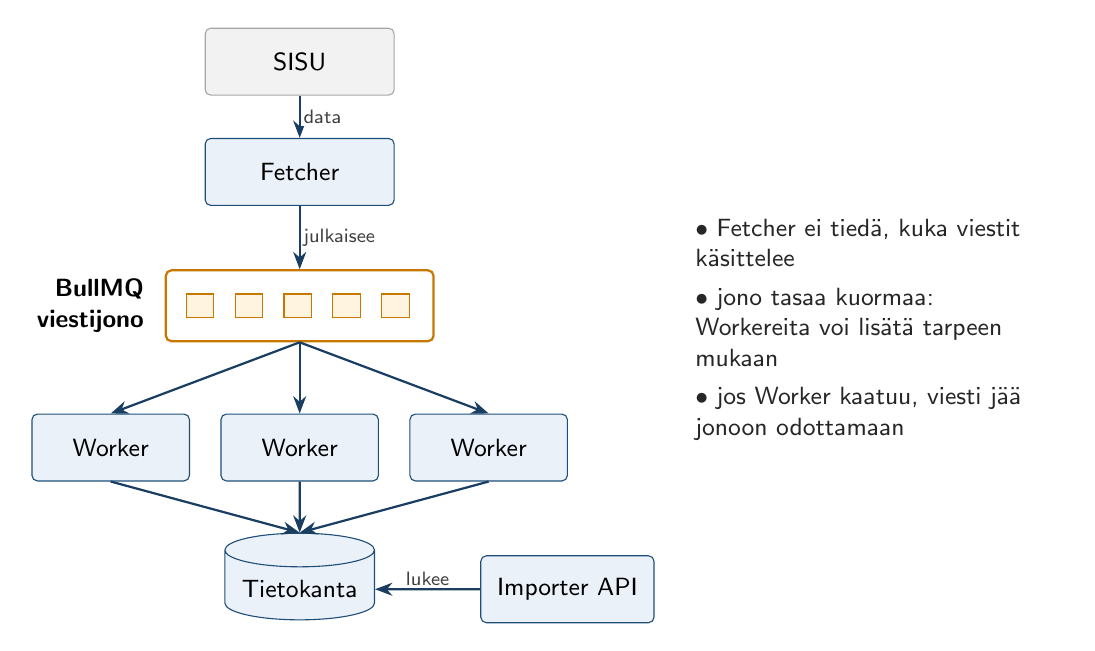
\begin{tikzpicture}[msg/.style={draw=oline,fill=ofill,minimum width=0.35cm,minimum height=0.3cm,inner sep=0pt}]
\node[ext,minimum width=2.4cm] (sisu) at (0,4.6) {SISU};
\node[box,minimum width=2.4cm] (fetch) at (0,3.2) {Fetcher};
% queue
\node[draw=oline,fill=white,thick,minimum width=3.4cm,minimum height=0.9cm,rounded corners=2pt] (q) at (0,1.5) {};
\foreach \i in {0,...,4} \node[msg] at ($(q.west)+(0.45+\i*0.62,0)$) {};
\node[font=\small\bfseries,left=4pt of q,align=right] {BullMQ\\viestijono};
\node[box,minimum width=2cm] (w1) at (-2.4,-0.3) {Worker};
\node[box,minimum width=2cm] (w2) at (0,-0.3) {Worker};
\node[box,minimum width=2cm] (w3) at (2.4,-0.3) {Worker};
\node[db] (db) at (0,-2.1) {Tietokanta};
\node[box,minimum width=2.2cm] (api) at (3.4,-2.1) {Importer API};
\draw[arr] (sisu) -- node[lbl,right] {data} (fetch);
\draw[arr] (fetch) -- node[lbl,right] {julkaisee} (q);
\foreach \w in {w1,w2,w3} {\draw[arr] (q.south) -- (\w.north); \draw[arr] (\w.south) -- (db.north);}
\draw[arr] (api) -- node[lbl,above] {lukee} (db);
\node[font=\small,text=gray!30!black,align=left,anchor=west,text width=4.6cm] at (4.9,1.2)
 {\raggedright\hyphenpenalty=10000 $\bullet$ Fetcher ei tiedä, kuka viestit käsittelee\\[3pt]
  $\bullet$ jono tasaa kuormaa: Workereita voi lisätä tarpeen mukaan\\[3pt]
  $\bullet$ jos Worker kaatuu, viesti jää jonoon odottamaan};
\end{tikzpicture}
\end{document}
